\documentclass{book}

\usepackage{graphicx,amscd,amsmath,amssymb,verbatim}
%\usepackage[dvips]{hyperref}	% for hyperlinks
\usepackage{url}
\usepackage{epstopdf} % so can use EPS or PDF figures
\usepackage{appendix}	% for finer control of the appendix

\DeclareMathSymbol{\Gamma}{\mathalpha}{letters}{"00}	% Greek capital letters in italics
\DeclareMathSymbol{\Delta}{\mathalpha}{letters}{"01}
\DeclareMathSymbol{\Theta}{\mathalpha}{letters}{"02}
\DeclareMathSymbol{\Lambda}{\mathalpha}{letters}{"03}
\DeclareMathSymbol{\Xi}{\mathalpha}{letters}{"04}
\DeclareMathSymbol{\Pi}{\mathalpha}{letters}{"05}
\DeclareMathSymbol{\Sigma}{\mathalpha}{letters}{"06}
\DeclareMathSymbol{\Upsilon}{\mathalpha}{letters}{"07}
\DeclareMathSymbol{\Phi}{\mathalpha}{letters}{"08}
\DeclareMathSymbol{\Psi}{\mathalpha}{letters}{"09}
\DeclareMathSymbol{\Omega}{\mathalpha}{letters}{"0A}

%%%%%%%%%%%%%%%%%%%%%%%%%%%%%%%%%%%%%%%%
%%%%%%%%%%%%%%%%%%%%%%%%%%%%%%%%%%%%%%%%
\begin{document}

\frontmatter

\begin{titlepage}
	\begin{center}

		\huge{Avalanches, Brains and Stocks: Simulating Self-Oraganised Criticality}

		\vspace{2.5cm}

		\LARGE{Avi Vajpeyi}\\ 
		\LARGE{Physics and Computer Science Departments}\\
		\LARGE{The College of Wooster}\\
		
		\vspace{0.5cm}
		
		\large A dissertation submitted in partial fulfillment 
		of the requirements of  Senior Independent Study in Physics at The College of Wooster\\
		
		\vspace{2.5cm}
		
		\begin{table}[h!]
			\begin{center}
				\begin{tabular}{c}
				
					\large{\emph{Physics Adviser}}\\
					\large{Dr. John F. Lindner}\\
					\vspace{0.5cm}\\
					\hline
					
					\vspace{1.0cm}\\
					\large{\emph{Computer Science}}\\
					\large{Dr. Denise Byrens}\\
					\vspace{0.5cm}\\
					\hline
					
				\end{tabular}
			\end{center}
		\end{table}
		
		\vspace{2.5cm}

		\large{\today}

	\end{center}
\end{titlepage}

%%%%%%%%%%%%%%%%%%%%%%%%%%%%%%%%%%%%%%%%
\chapter*{Abstract}\addcontentsline{toc}{chapter}{Abstract}
\indent Experiments with a granular bead pile have shown that the pile can model critical systems such as avalanches. In the experiments, a bead is dropped on the apex of the pile of beads. Eventually, one such bead causes several beads of the conical bead pile to avalanche. The experiments have studied the distribution of avalanches and how the distribution is affected by altering the bead type, bead cohesion, and bead drop height. In this study we present a computational simulation of the experiment. The simulation models each bead as independent particles with their own positions and velocities. The internal and external forces on each particle are accumulated to provide the new particle positions using Newton's second law of motion. The independence of each particle allows a natural way to express parallelism which we utilise by threading various processes of the particles to the graphical processing unit. This allows the simulation run in real-time while still having $60$k particles on the pile.\\
\indent With this simulation we can learn new information from the system that may have been challenging to study with the actual experiment. For example, we can vary the shapes and numbers of the beads. With the simulation it is also possible to record the velocity of each particle on the surface and even inside the pile. 

%%%%%%%%%%%%%%%%%%%%%%%%%%%%%%%%%%%%%%%%
%\chapter*{Acknowledgments}\addcontentsline{toc}{chapter}{Acknowledgments}
%I would like to thank Dr. Lindner and Dr.

%%%%%%%%%%%%%%%%%%%%%%%%%%%%%%%%%%%%%%%%
%%%%%%%%%%%%%%%%%%%%%%%%%%%%%%%%%%%%%%%%
\tableofcontents
\setcounter{tocdepth}{2}
\listoftables
\listoffigures

%%%%%%%%%%%%%%%%%%%%%%%%%%%%%%%%%%%%%%%%
%%%%%%%%%%%%%%%%%%%%%%%%%%%%%%%%%%%%%%%%
%%%%%%%%%%%%%%%%%%%%%%%%%%%%%%%%%%%%%%%%
\mainmatter

%%%%%%%%%%%%%%%%%%%%%%%%%%%%%%%%%%%%%%%%
%%%%%%%%%%%%%%%%%%%%%%%%%%%%%%%%%%%%%%%%
\chapter{Introduction}\label{introduction}
%discussion of everything in shallow... 
\section{Per Bak and Sand in Brains}
In 1999 a Danish Scientist by the name Per Bak explained the disordered electrical neural activity of a brain in an audacious way that left many neurologists puzzled.  He suggested that the brain's neural activity worked in a similar procedure as a sand pile which incur avalanches of varying sizes to maintain stability (instabilities paradoxically helping provide the system with stability). As more sand is added to the pile, more avalanches occur along the surface of the conical shape. Even with these unpredictable surface avalanches, the conical shape of the pile is maintained. Per Bak pointed out that although the individual avalanches were unpredictable in timing and size, the \textit{distribution} of the timings and sizes of several avalanches \textit{demonstrate a regularity}. He termed this phenomena of finding order in systems which appeared to be unpredictable with a term he created - ``self-organised criticality'' (SOC).  He explained to the neurologists that perhaps brains, like sand piles, behave as a self organised critical system. This is because the ordered complexity in a brain which permits the ability to think arises spontaneously from the disordered electrical activity of neurons .


\section{The Origins of SOC: Tipping Points}
In the 1980s, Bak began studying phase transitions in the hopes of better understanding how it is possible to find order in nature which is constituted by a disordered assortment of particles. Phase transitions, the process in which matter transforms from one phase to another, can involve a sudden change, like the magnetization of ferro-magnets, or can involve a gradual change, like ice transitioning to water. In any transition, there is a precise moment called the tipping or critical point at which the matter is halfway between each phase. In the case for most phase transitions, there are certain criteria that need to be met before matter can transition to another phase. For example -- the local temperate and pressure must be within a specific range for ice to transition into water. Studying these transitions which are dependent on the surrounds to occur lead Bak to question transitions which were able to occur spontaneously. He observed that in spontaneously phase transitioning systems, interactions of local elements of the system could spontaneously bring the system to a critical point -- a self oraganised critical point. 
In 1987 Per Bak and a group of his colleagues published the first paper on SOC and soon afterward, Bak even published a book titled \textit{`How Nature Works'}. In the book, Bak extends the concept of SOC and demonstrates its presence in other complex systems ranging from financial markets,  coastline formation, evolution, earthquakes, galaxy distributions and even the brain. According to Bak, these systems hover between the fence separating order from disorder. Bak was able to study these only with simulations and so other scientists were still skeptical of his hypotheses about SOC.

However, in 1992, the physics department of the University of Oslo was able to experimentally test Bak's sand pile model.

One of the first empirical tests of Bak’s sand pile model took place in 1992, in the physics department of the University of Oslo. The physicists confined piles of rice between glass plates and added grains one at a time, capturing the resulting avalanche dynamics on camera. They found that the piles of elongated grains of rice behaved much like Bak’s simplified model.
Most notably, the smaller avalanches were more frequent than the larger ones, following the expected power law distribution. That is, if there were 100 small avalanches involving only 10 grains during a given time frame, there would be 10 avalanches involving 100 grains in the same period, but only a single large avalanche involving 1,000 grains. (The same pattern had been observed in


\section{The Experiment}

\section{Simulation}
\subsection{Previous Work}
\subsection{Speed Boosts with GPUs}
\subsection{Unified Particle Physics and Position Based Dynamics}


\section{Overview of Thesis}


\chapter{Theory}
\section{Physics of the Experimental System}
\subsection{SOC and the power Law}
\subsubsection{Effect of Drop Height}
\subsubsection{Effect of Cohesion}
\subsection{Angle of Repose}
\subsection{Cohesion between Beads}

\section{How to take Advantage of GPUs}
\subsection{GPUs traditional role in Computers}
\subsection{Parallelising Code and Threading}

\section{Algorithms Used}
\subsection{Boundary Volume Hierarchy}
\subsection{Position-Based Dynamics}
\subsection{Unified-Particle Solving}

\chapter{Results}
\section{Comparing Simulation to Experiment}
\section{Novel Results}

\chapter{}

% %%%%%%%%%%%%%%%%%%%%%%%%%%%%%%
\section{Math \& Citations}	% "&" is a special character
Examples of inline math are $\alpha = \sqrt{\gamma^2 + \Gamma^2}$ and $\vec{v} = 7 \hat{x} - 5 \hat{y}$ and $\vec u \times \vec v$ and $c = (2.99 \pm 0.01) \times 10^8$ m/s. One example of block (display) math is
%
\begin{equation}
	\int_0^1x^2 dx = \frac{1}{3},
	\label{myIntegral}
\end{equation}
%
and a second example is
%
\begin{equation}
	\xi = \alpha \left( \frac{1}{ \omega_0^2 + \omega^2 } \right).
	\label{signal}
\end{equation}
%
Note how block math is punctuated like words in a sentence! The block math equations are automatically numbered. We can reference Eq. \ref{myIntegral} or Eq. \ref{signal} by inserting labels in the block, but then we must compile \LaTeX\ twice.

We can readily cite articles \cite{Chenciner2000}  and books \cite{Gleick1987} and URLs \cite{Lindner2015} in our bibliography, but now we must compile \LaTeX, Bib\TeX,  \LaTeX, \LaTeX.

% %%%%%%%%%%%%%%%%%%%%%%%%%%%%%%
\section{Figures \& Tables}
We can also include figures, but first we need to use package ``graphicx" under document class. We can reference Fig. \ref{SchematicDiagram} like equations. All figures should have captions.

\begin{figure}[ht] % "ht" = here or top
	\begin{center}
		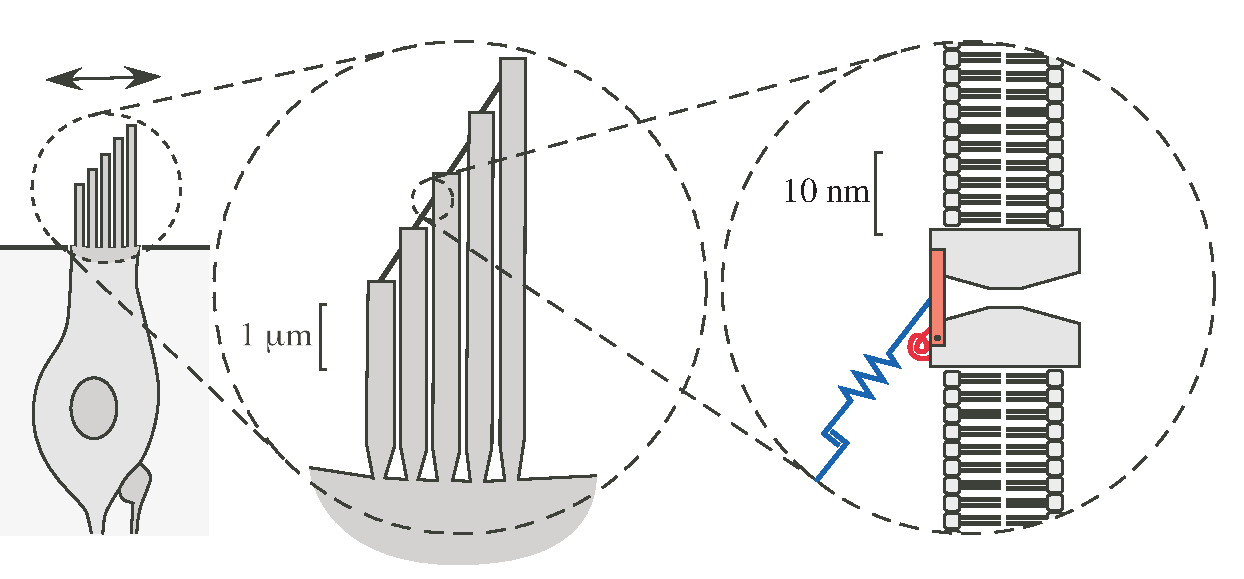
\includegraphics[width=0.8\linewidth]{Figures/ExampleFigure} % For Mac OS X PDFs (else append .eps)
		\caption{Figure captions go on bottom.}
		\label{SchematicDiagram}
	\end{center}
\end{figure}

Finally, we can also include tables, such as Table \ref{demoTable}. Like figures, we can also \emph{attempt} to force their positions. 

In the document class line, we can easily convert from ``preprint" one-column, double-spacing for rough drafts to ``twocolumn" single spacing for final drafts! 

This is dummy text. This is dummy text. This is dummy text. This is dummy text. This is dummy text. This is dummy text. This is dummy text. This is dummy text. This is dummy text. This is dummy text. This is dummy text. This is dummy text. This is dummy text. This is dummy text. This is dummy text. This is dummy text. This is dummy text. This is dummy text. This is dummy text. This is dummy text. This is dummy text. This is dummy text. This is dummy text. This is dummy text. This is dummy text. This is dummy text. 

\begin{table}[h] % indenting is optional	
	\caption{Table captions go on top.}
	\label{demoTable}
	\begin{center}
		\begin{tabular}{cc} % "cc" = center each column
			absicssa & ordinate\\
			\hline
			1.0 s & 5.6 m\\
			2.0 s & 6.7 m\\
			3.0 s & 9.9 m
		\end{tabular}
	\end{center}
\end{table}

%%%%%%%%%%%%%%%%%%%%%%%%%%%%%%%%%%%%%%%%
%%%%%%%%%%%%%%%%%%%%%%%%%%%%%%%%%%%%%%%%
\chapter{Conclusions}\label{Conclusions}

\section{Stuff}
This is dummy text. This is dummy text. This is dummy text. This is dummy text. This is dummy text. This is dummy text. This is dummy text. This is dummy text. This is dummy text. This is dummy text. This is dummy text. This is dummy text. This is dummy text. This is dummy text. This is dummy text. This is dummy text. This is dummy text. This is dummy text. This is dummy text. This is dummy text. This is dummy text. This is dummy text. This is dummy text. This is dummy text. This is dummy text. This is dummy text. 

This is dummy text. This is dummy text. This is dummy text. This is dummy text. This is dummy text. This is dummy text. This is dummy text. This is dummy text. This is dummy text. This is dummy text. This is dummy text. This is dummy text. This is dummy text. This is dummy text. This is dummy text. This is dummy text. This is dummy text. This is dummy text. This is dummy text. This is dummy text. This is dummy text. This is dummy text. This is dummy text. This is dummy text. This is dummy text. This is dummy text. 


%%%%%%%%%%%%%%%%%%%%%%%%%%%%%%%%%%%%%%%%
%%%%%%%%%%%%%%%%%%%%%%%%%%%%%%%%%%%%%%%%
\appendix

\noappendicestocpagenum	 % suppress page number ...
\addappheadtotoc	% ... but add appendices header to table of contents 

\renewcommand{\theequation}{A-\arabic{equation}} % redefine the command that creates the equation number
\setcounter{equation}{0}  % reset counter 

\renewcommand{\thesection}{A-\arabic{section}} % redefine the command that creates the section number
\setcounter{section}{0}  % reset counter 

\renewcommand{\thetable}{A-\arabic{table}} % redefine the command that creates the table number
\setcounter{table}{0}  % reset counter 

%%%%%%%%%%%%%%%%%%%%%%%%%%%%%%%%%%%%%%%%
%%%%%%%%%%%%%%%%%%%%%%%%%%%%%%%%%%%%%%%%
\chapter{Extra Stuff}\label{Extra}

This is dummy text. This is dummy text. This is dummy text. This is dummy text. This is dummy text. This is dummy text. This is dummy text. This is dummy text. This is dummy text. This is dummy text. This is dummy text. This is dummy text. This is dummy text. This is dummy text. This is dummy text. This is dummy text. This is dummy text. This is dummy text. This is dummy text. This is dummy text. This is dummy text. This is dummy text. This is dummy text. This is dummy text. This is dummy text. This is dummy text. 

This is dummy text. This is dummy text. This is dummy text. This is dummy text. This is dummy text. This is dummy text. This is dummy text. This is dummy text. This is dummy text. This is dummy text. This is dummy text. This is dummy text. This is dummy text. This is dummy text. This is dummy text. This is dummy text. This is dummy text. This is dummy text. This is dummy text. This is dummy text. This is dummy text. This is dummy text. This is dummy text. This is dummy text. This is dummy text. This is dummy text. elegant text. This elegant text. This elegant text. This elegant text. This elegant text. 

%%%%%%%%%%%%%%%%%%%%%%%%%%%%%%%%%%%%%%%%
%%%%%% *-%%%%%%%%%%%%%%%%%%%%%%%%%%%%%%%%%
\chapter{Extra Stuffing}\label{Stuffing}
This is dummy text. This is dummy text. This is dummy text. This is dummy text. This is dummy text. This is dummy text. This is dummy text. This is dummy text. This is dummy text. This is dummy text. This is dummy text. This is dummy text. This is dummy text. This is dummy text. This is dummy text. This is dummy text. This is dummy text. This is dummy text. This is dummy text. This is dummy text. This is dummy text. This is dummy text. This is dummy text. This is dummy text. This is dummy text. This is dummy text. 

This is dummy text. This is dummy text. This is dummy text. This is dummy text. This is dummy text. This is dummy text. This is dummy text. This is dummy text. This is dummy text. This is dummy text. This is dummy text. This is dummy text. This is dummy text. This is dummy text. This is dummy text. This is dummy text. This is dummy text. This is dummy text. This is dummy text. This is dummy text. This is dummy text. This is dummy text. This is dummy text. This is dummy text. This is dummy text. This is dummy text. 

%%%%%%%%%%%%%%%%%%%%%%%%%%%%%%%%%%%%%%%%
%%%%%%%%%%%%%%%%%%%%%%%%%%%%%%%%%%%%%%%%
%%%%%%%%%%%%%%%%%%%%%%%%%%%%%%%%%%%%%%%%
\backmatter

\addcontentsline{toc}{chapter}{Bibliography}
\bibliography{thesis}
%\bibliographystyle{plain}			% listed alphabetically but ordered numerically, including titles
\bibliographystyle{unsrt}			% like plain but references appear in order of citation
%\bibliographystyle{alpha}		% like plain, except reference labels used
%\bibliographystyle{abbrv}		% like plain, but abbreviations uses for authors first names, etc.

\end{document}